\documentclass[twocolumn]{article}
\usepackage{graphicx} % Required for inserting images
\usepackage{subfig}
\usepackage{amsmath}
\usepackage{subcaption}
\usepackage[hyphens]{url}
\usepackage{hyperref}
\usepackage{tikz}
\usetikzlibrary{chains,shadows.blur}
\hypersetup{breaklinks=true}

\urlstyle{same}

\pagenumbering{gobble}
\title{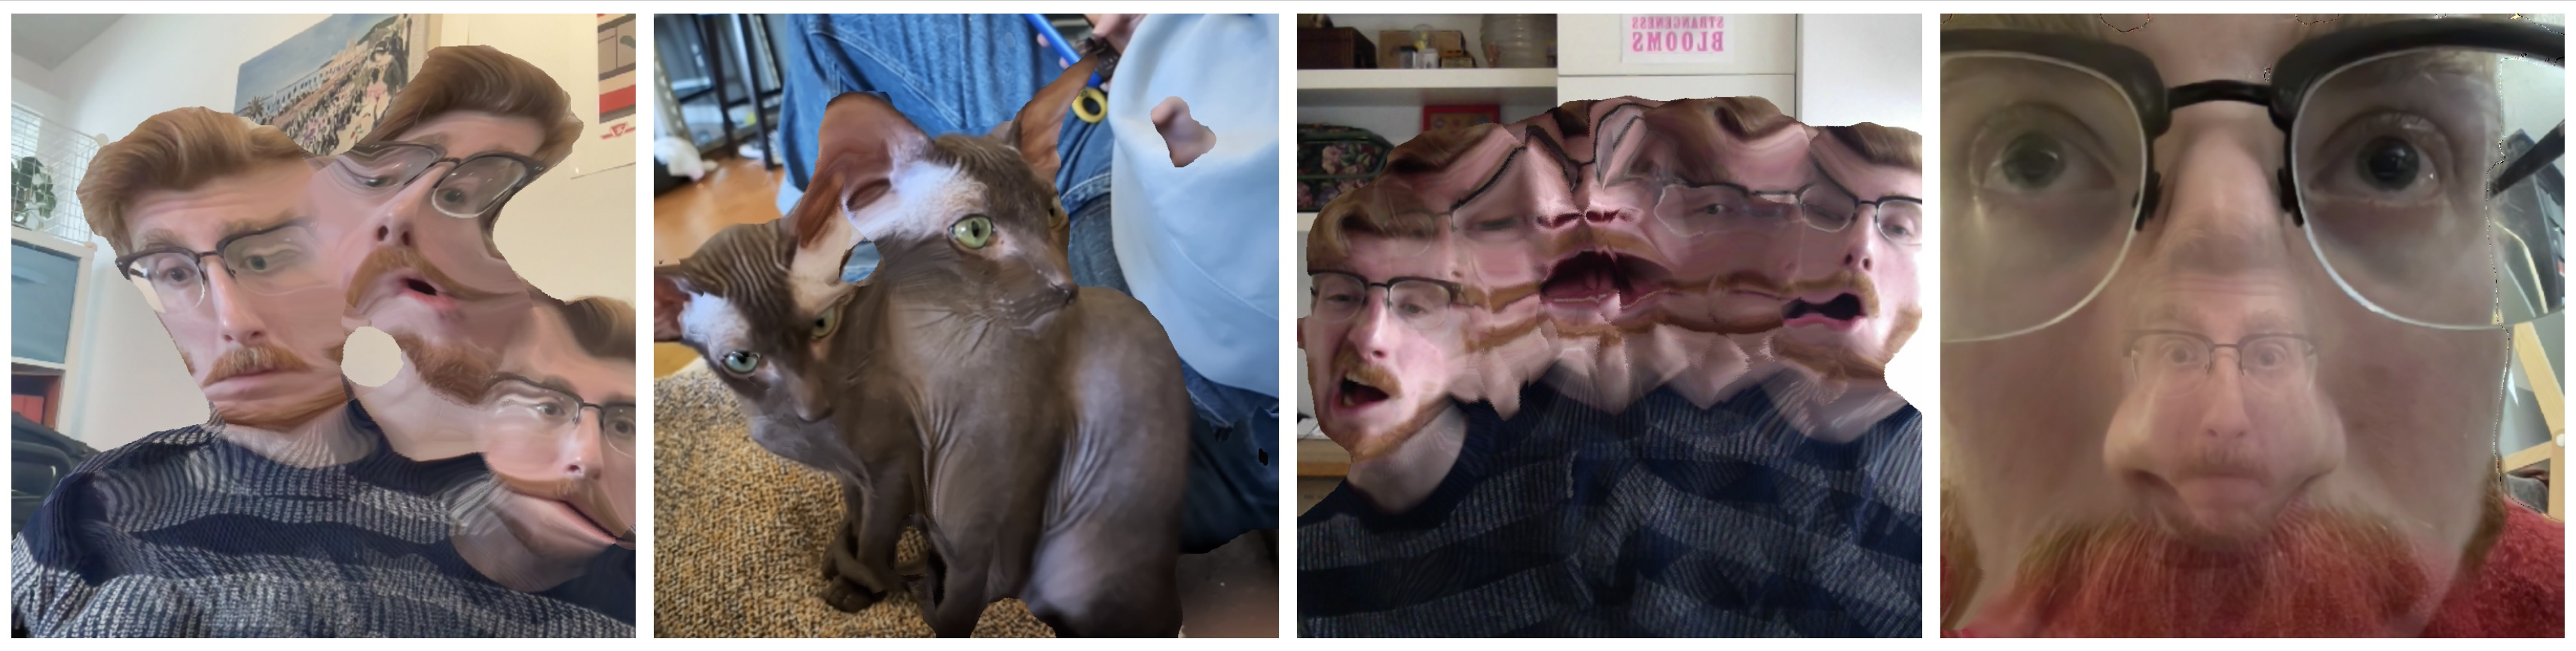
\includegraphics[width=\textwidth]{img/teaser.jpg}\\ Pandemonium: A Panorama App to Maximize Jank}
\author{Dave Pagurek}
\date{March 2025}

\begin{document}

\maketitle

\begin{abstract}
    The panorama feature on early smartphones produced frequent delightful visual glitches. Modern panorama apps are better at accurately reproducing their subjects, and subsequently forget their true goal: surprising the user with the unexpected and uncanny. We propose a novel camera system that maximizes occurrences of weird visuals rather than trying to sweep them under the rug.
\end{abstract}

\section{Introduction}

Who doesn't want to see their cat have eight legs?~\cite{cheezburger} Panoramas used to provide a steady source of delight as subjects inevitably move while the panorama is being captured, such as the cat in Figure~\ref{fig:cat}. We refer to these glitches as \textit{jank.} While jank still occurs in the capture phase of modern panorama apps, the final image disappointingly removes most jank.

App makers have lost sight of their true goal: producing images that inspire a sense of biblical awe. Like how paintings got weird and embraced the surreal and abstract once photographs became common, panoramas too need to get weird now that it's easy to capture reality.

We aim to fill this niche. First, we explore what used to produce panorama jank. We then design a new camera system optimized for jank. Finally, we evaluate this system by exploring its effectiveness at producing surprising results in the hands of users.

\begin{figure}
    \centering
    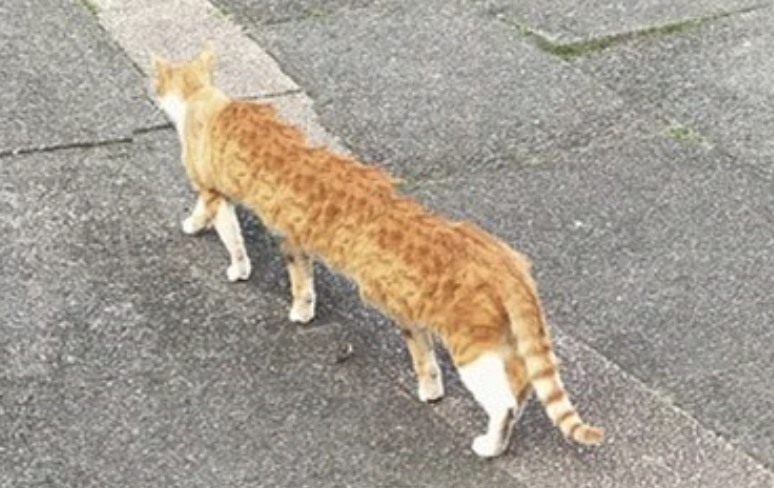
\includegraphics[width=0.78\linewidth]{img/cat-pano.png}
    \caption{A panorama of a cat featuring more limbs than typically expected.~\cite{cheezburger}}
    \label{fig:cat}
\end{figure}

\section{Background}

\begin{figure}
    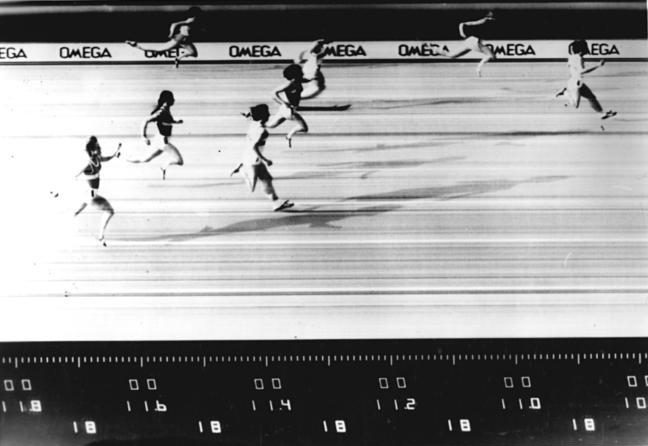
\includegraphics[width=0.98\linewidth]{img/photofinish.jpg}
    \caption{Finish photo of a world record 100m run by Marlies Oelsner, 1 July 1977.~\cite{photofinish} The ``OMEGA'' text in the background appears undistorted because it was moving horizontally over time.}
    \label{fig:photofinish}
\end{figure}

\textit{Slit scanning} is a photography technique where a full, two-dimensional image is created by scanning a series of one-dimensional images over time. This is used for photo finishes in sports, such as the one in Figure~\ref{fig:photofinish}. The camera only sees the vertical finish line. As the film slides through the camera horizontally, that single vertical line is stretched across the full frame. Although the slit captures the same space, the time varies, allowing one to easily see who crosses the finish line first first by seeing who appears first horizontally. It also has the side effect of distorting everything that isn't moving purely horizontally, leading to curvy and stretched limbs.

Slit scanning is similar to how digital cameras take photos. Unlike slit scanning, each pixel is looking at a different position in space, but each row of pixels gets exposed with a slight time offset from the row preceding it. This leads to an effect called \textit{rolling shutter}: fast-moving objects like airplane propellors appear distorted, and if the camera itself is moving, video looks wiggly and jello-like.~\cite{wikipedia-contributors-2024}

Old panorama apps work by adding columns of pixels to the image as the user pans the camera.~\cite{kuehnel-2012} Like rolling shutter, this means adjacent pixels are offset in time. Any point where adjacent pixels have a time offset introduces a temporal ``seam'' where changes in time of the subject turn into spatial variations in the resulting image.

Modern panorama apps in the ``photo sphere'' style, rather than making the user take one continuous scan, allow discrete snapshots to be taken at the user's leasure. This makes it easier to plan and compose a panorama, but unfortunately greatly reduces the number of temporal seams where jank might appear.

\section{Characteristics of Jank}
\label{sec:characteristics}

These are the types of jank that can appear in a traditional panorama, and how they come to be. These are the visual properties we hope to replicate.

\paragraph{Duplication.} If an object gets scanned, and then moves into the path of the scan again, it can get scanned a second time, showing up multiple times in the resulting image. This is what has happened to the cat's legs in Figure~\ref{fig:cat}.

\paragraph{Bend.} Even if an object moves rigidly over time, if its velocity is nonlinear, it will appear spatially nonlinear in a panorama. This can result in objects looking rubbery and curvy. The legs of the runners in Figure~\ref{fig:photofinish} show this, especially the one in the top left.

\paragraph{Smear.} Objects that move in the same direction of the camera get stretched out. Objects that move in the opposite direction get squished. Figure~\ref{fig:smearpano} demonstrates some extreme examples of this.

\begin{figure}
    \centering
    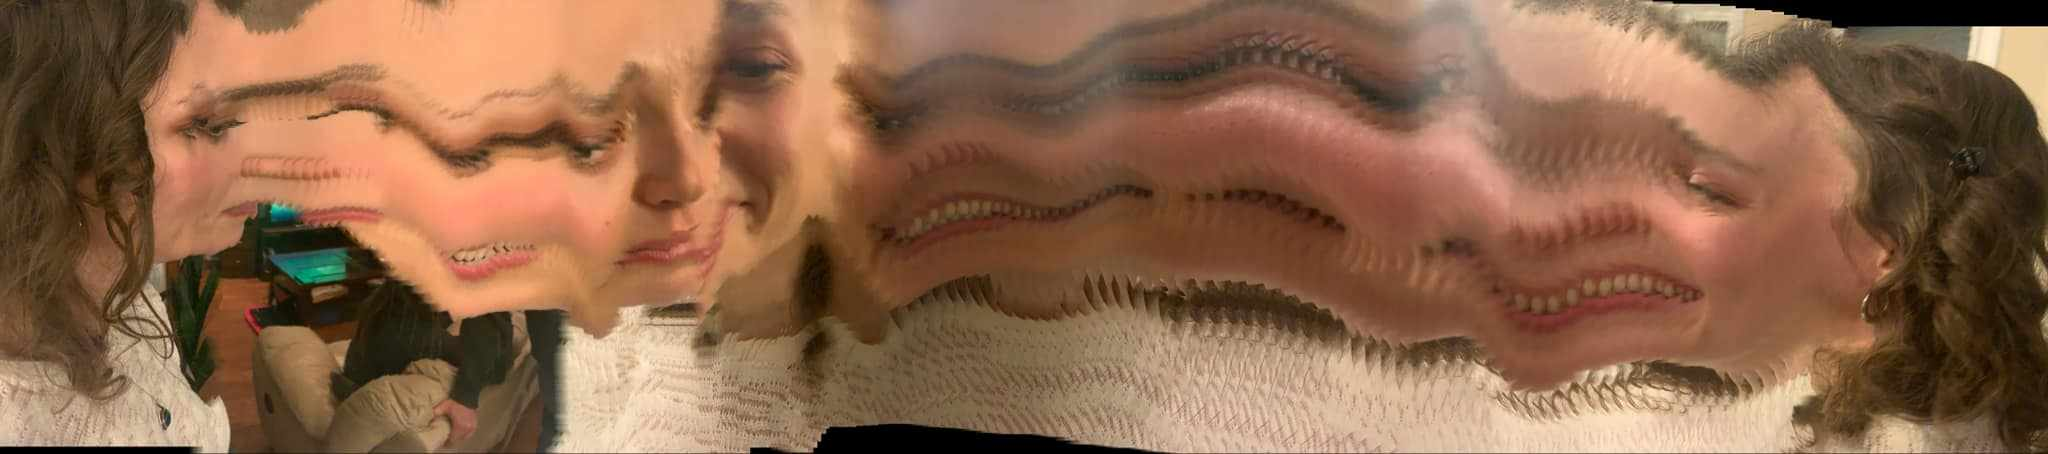
\includegraphics[width=0.98\linewidth]{img/badpano2.jpg}
    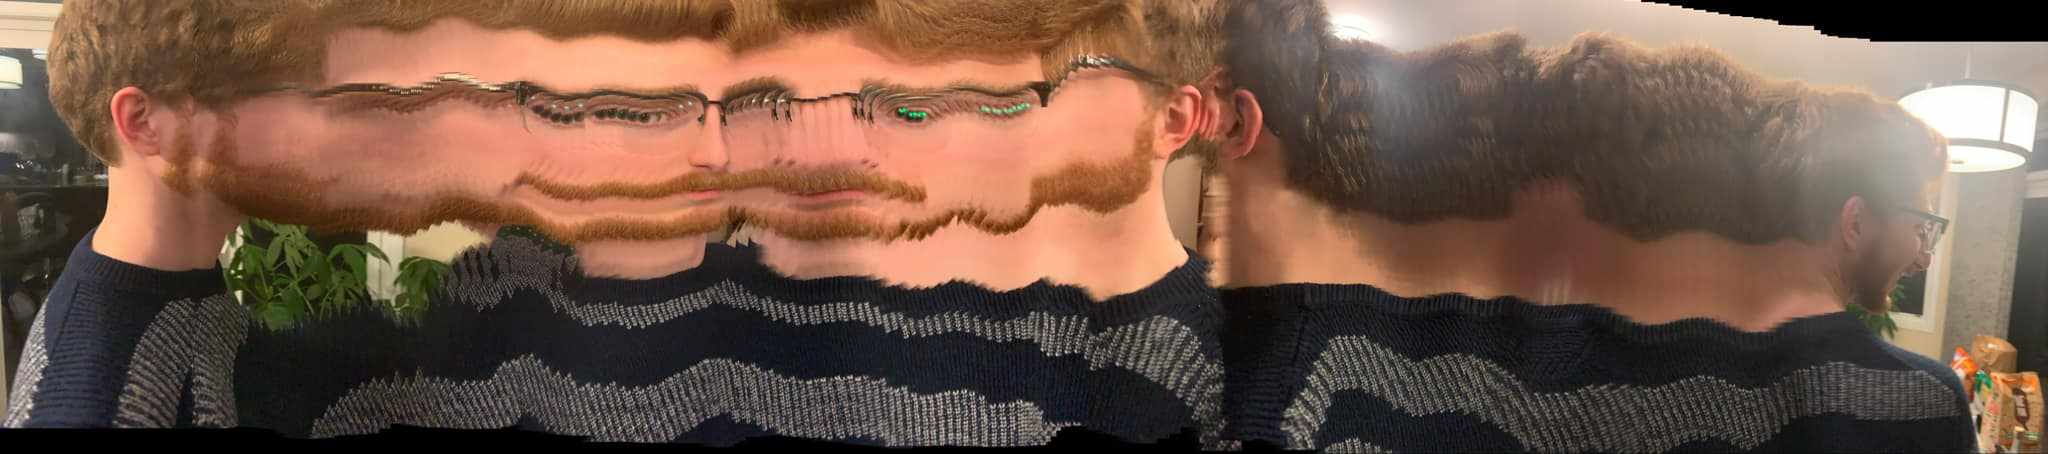
\includegraphics[width=0.98\linewidth]{img/badpano3.jpg}
    \caption{Smear jank in a slit scan panorama caused by a subject moving with the camera as it pans while also rotating in place.}
    \label{fig:smearpano}
\end{figure}

\section{Method}

Pandemonium allows users to build up a composite incrementally by stamping content piece by piece. Each additive stamp contains only the isolated foreground from the camera, with random sinusoidal distortion applied, and is smoothly blended with the previous content.

The distortion on stamps creates \textbf{bend jank.} Repeated stamping of the same object creates \textbf{duplication jank.} The smooth blending creates \textbf{smear jank} at the seams of stamps.


\begin{figure}
    \centering
    \subfloat[Input 1]{
        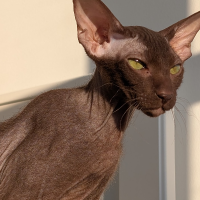
\includegraphics[width=0.33\linewidth]{img/step-1-1.png}
    }
    \subfloat[Segmented]{
        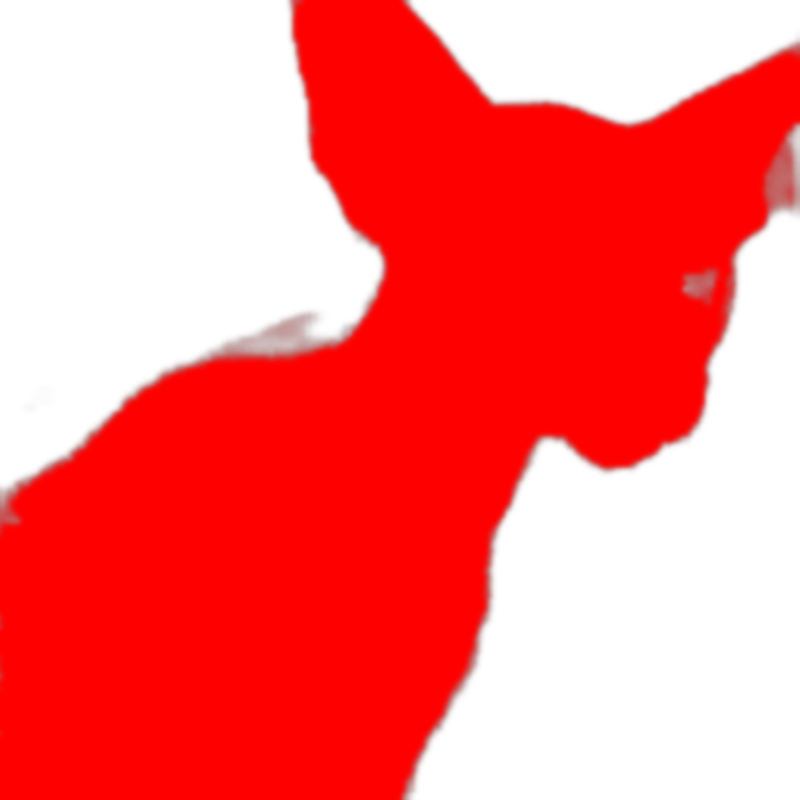
\includegraphics[width=0.33\linewidth]{img/step-1-2.png}
    }
    \subfloat[Warped]{
        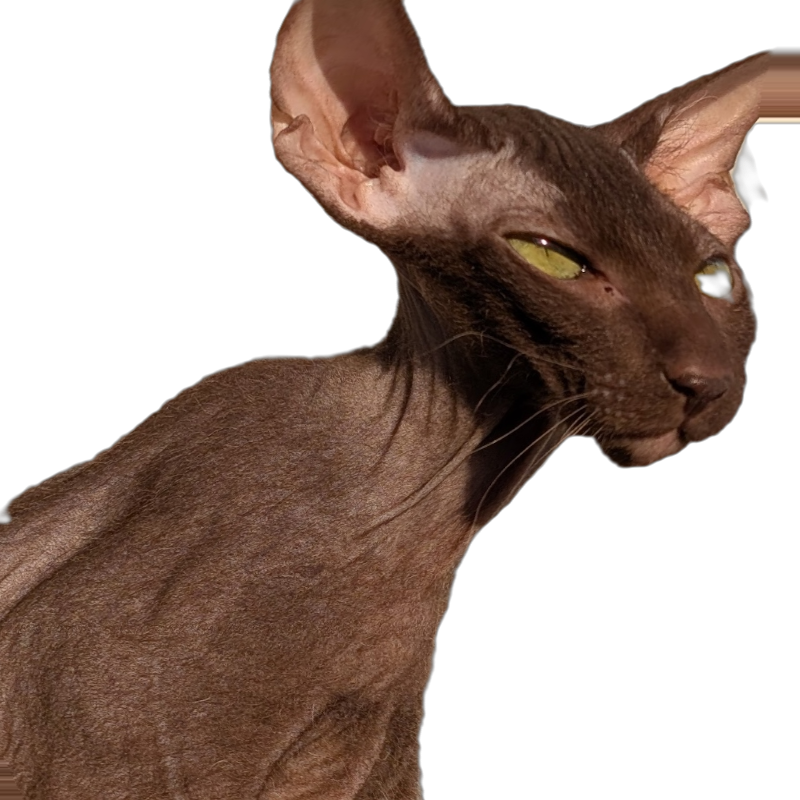
\includegraphics[width=0.33\linewidth]{img/step-1-3.png}
    }
    \hfill
    \subfloat[Input 2]{
        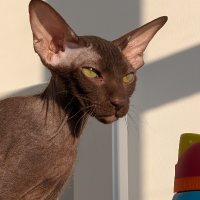
\includegraphics[width=0.33\linewidth]{img/step-2-1.png}
    }
    \subfloat[Segmented]{
        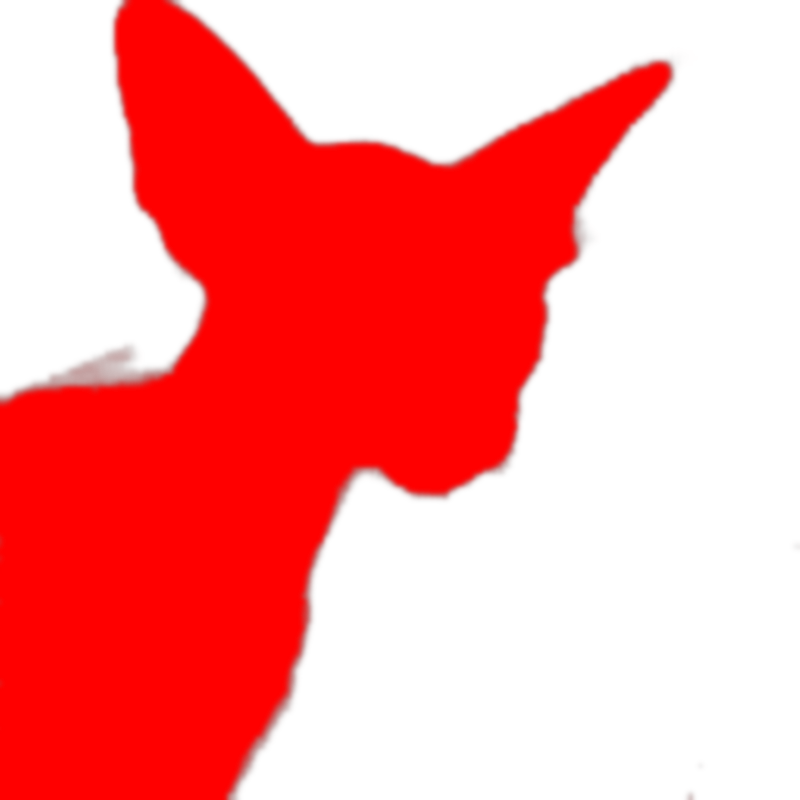
\includegraphics[width=0.33\linewidth]{img/step-2-2.png}
    }
    \subfloat[Warped]{
        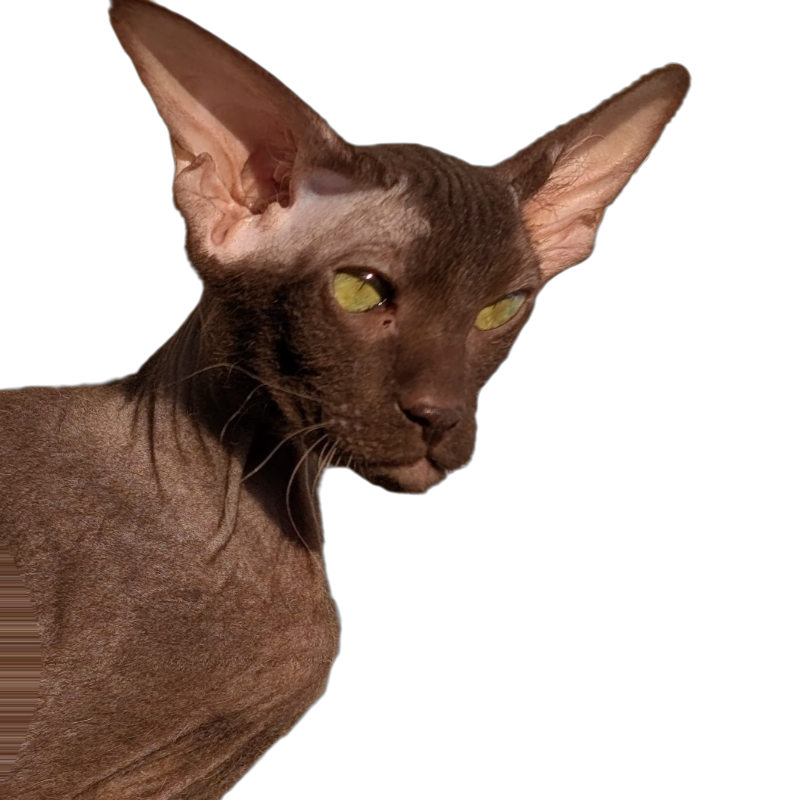
\includegraphics[width=0.33\linewidth]{img/step-2-3.png}
    }
    \hfill
    \subfloat[Distance to edge]{
        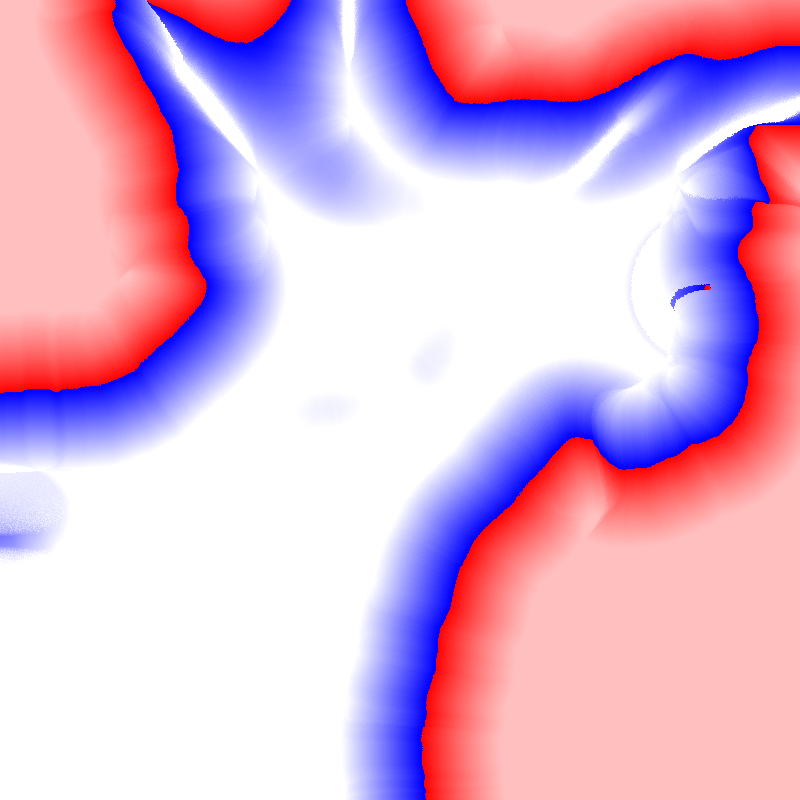
\includegraphics[width=0.33\linewidth]{img/step-2-4.png}
    }
    \subfloat[Input 1 Seams]{
        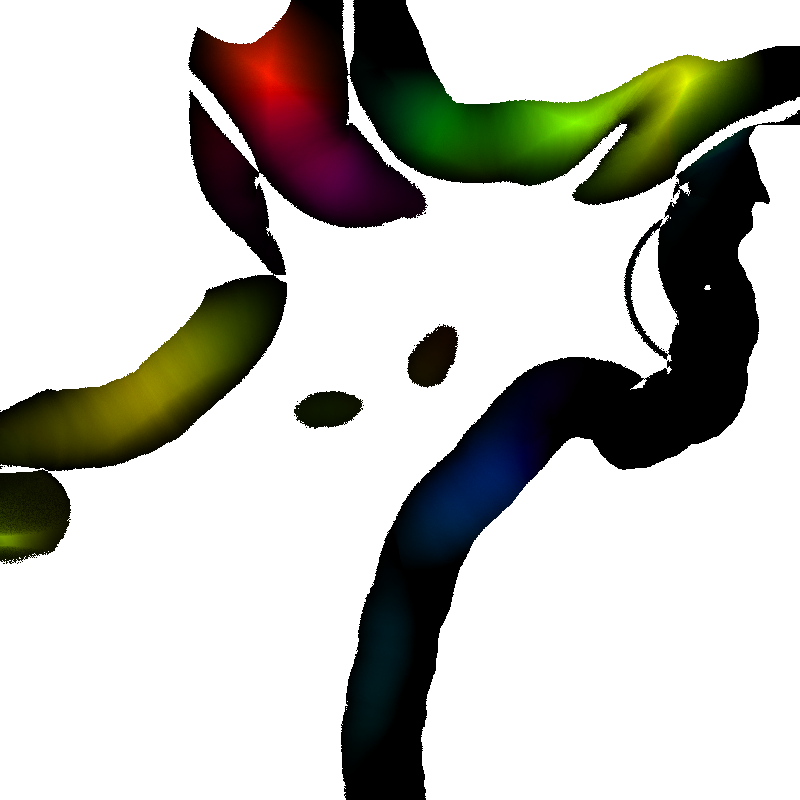
\includegraphics[width=0.33\linewidth]{img/step-2-5.png}
    }
    \subfloat[Input 2 Seams]{
        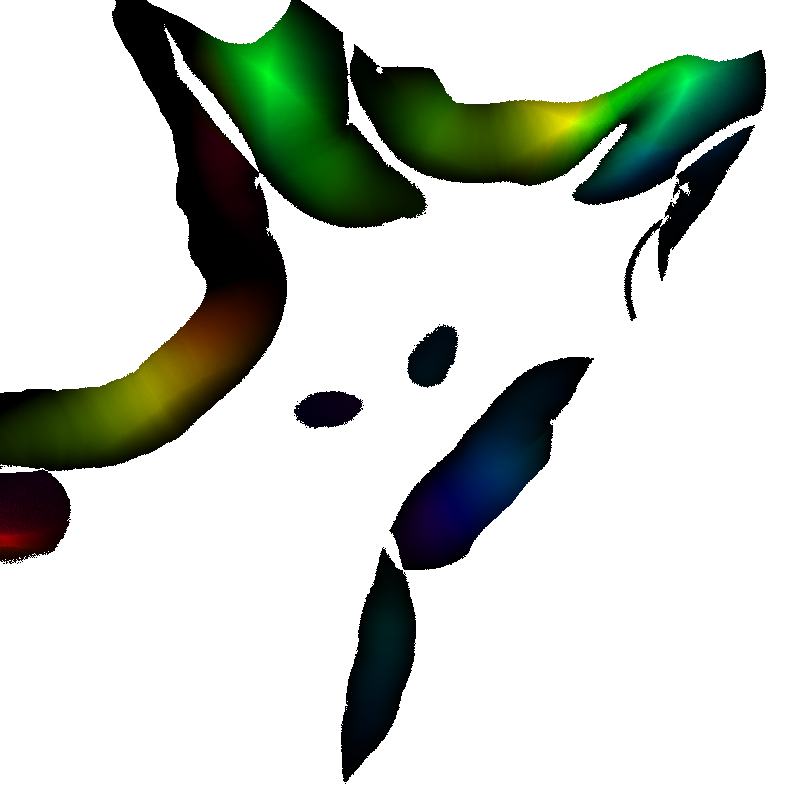
\includegraphics[width=0.33\linewidth]{img/step-2-6.png}
    }
    \hfill
    \subfloat[Final composite]{
        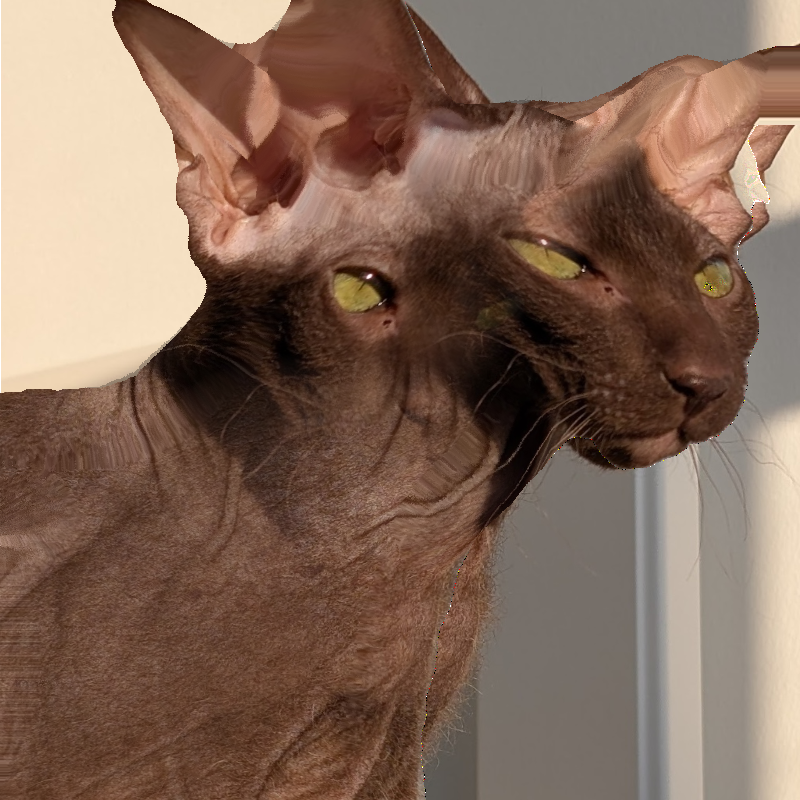
\includegraphics[width=0.5\linewidth]{img/cat-composite.png}
    }
    \caption{Given inputs (a) and (d): (b) and (e) show masks separating foreground from background; (e) and (f) show applied warp; (g) shows signed distance to the joint shape (inside is blue, outside is red); (h) and (i) show the regions from each input on the seams between the two inputs that need to smear (hue angle indicates direction, brightness indicates magnitude of smear.) The final image is shown in (j).}
    \label{fig:steps}
\end{figure}


\subsection{Flow}

The app keeps track of three image buffers: the background layer, the foreground layer, and the ``scratch'' layer previewing what the result will be when a snapshot is taken. The background layer captures the camera in the first snapshot. On the scratch layer, we preview the result of stamping the snapshot. When a snapshot is taken, we simply replace the foreground layer with the scratch buffer. Figure~\ref{fig:controlflow} shows this process in a control flow diagram.

When creating a composite, we run the camera feed through \textsc{Segment}(), which isolates the foreground from the background. We then run the result through \textsc{Warp}(), which applies a sinusoidal offset to the pixels. Finally, we combine the result with the current foreground layer using \textsc{Amalj}(), the jank amalgamate or ``amaljamate'' operator.

\begin{figure}
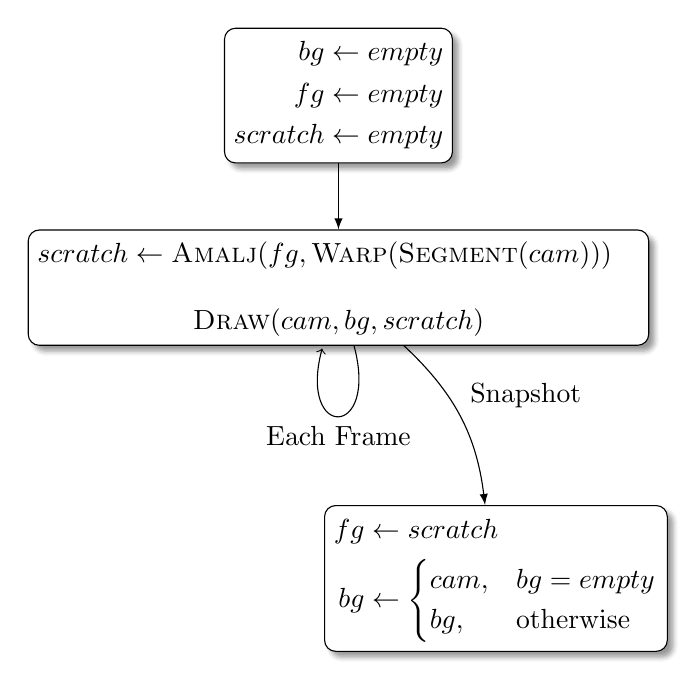
\begin{tikzpicture}[auto,
  node distance = 12mm,
  start chain = going below,
  box/.style = {draw,rounded corners,blur shadow,fill=white,
        on chain,align=center}]
 \node[box] (b1)    {$\begin{aligned}bg &\leftarrow empty \\
 fg &\leftarrow empty \\
 scratch &\leftarrow empty\end{aligned}$}; 
 \node[box] (b2) at (0, -0.5)   {$\begin{aligned}
 scratch &\leftarrow \textsc{Amalj}(fg, \textsc{Warp}(\textsc{Segment}(cam)))\end{aligned}$ \\
 \\
 $\textsc{Draw}(cam, bg, scratch)$};
 \node[box] (b3) at (2, -4)    {$\begin{aligned}fg &\leftarrow scratch \\
 bg &\leftarrow \begin{cases}
 cam, &bg = empty\\
 bg, &\text{otherwise}
 \end{cases}
 \end{aligned}$};  
 \begin{scope}[rounded corners,-latex]
  %\path %(b2.-40) edge[bend left=50] (b4.40);
  \path (b1) edge (b2);
  \path (b2) edge[bend left=20] node {Snapshot} (b3);
  \path (b2) edge [loop below] node {Each Frame} (b2);
  %(b2.-40) edge[bend left=50] (b2.40);
  % \draw (b3.230) -- ++(0,-0.3) -| ([xshift=-5mm]b2.west) |-
  % ([yshift=3mm]b2.130) -- (b2.130);
 \end{scope}
\end{tikzpicture}
\caption{Pandemonium control flow.}
\label{fig:controlflow}
\end{figure}

\subsection{Segmentation}
The \textsc{Segment}() function applies the MediaPipe body segmentation model~\cite{selfie-segmentation} to isolate the subject. The result is an image with just the foreground on a transparent background. The segmentation mask is shown in Figure~\ref{fig:steps}b,e.

\subsection{Warp}
The \textsc{Warp}() function applies a horizontal sinusoidal offset to each pixel in the image. The amplitude and frequency of the offset is controlled by a single parameter $w \in [0,1]$ for simplicity, and a constant $c \in [0, 2\pi]$ that is randomly picked for each snapshot:

\begin{equation}
    x' = x + 0.1w\sin(20wy+c)
\end{equation}

The warped foreground elements are shown in Figure~\ref{fig:steps}c,f.

\subsection{Amaljamate Operator}

Our amaljamate operator is designed to run in a fragment shader in WebGL, and therefore is defined as a function run for each pixel coordinate, outputting a final merged pixel color.

Its high level goal is to merge two subjects. If the two subjects are far apart, they should appear unchanged. The goal, shown  in Figure~\ref{fig:merge}, is that as they grow closer together, they start to smear into each other. As they touch and combine, their smeared colors blend smoothly into each other. When two subjects fully overlap, shown in Figure~\ref{fig:overlap}, they have a seam all around the subjects' exteriors, leaving only the middle is undistorted.

\begin{figure}
    \centering
    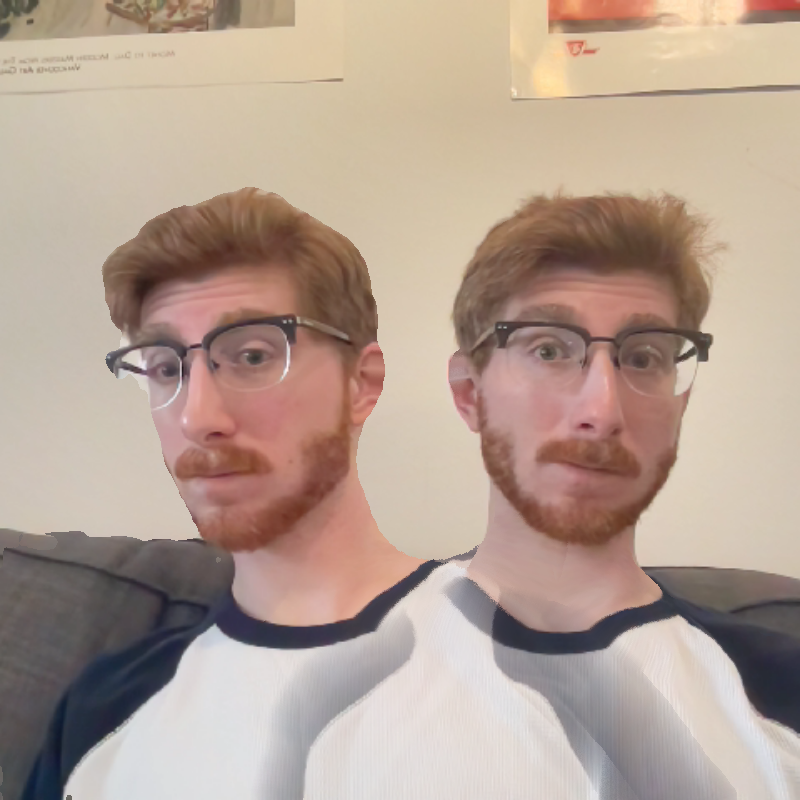
\includegraphics[width=0.45\linewidth]{img/merge1.png}
    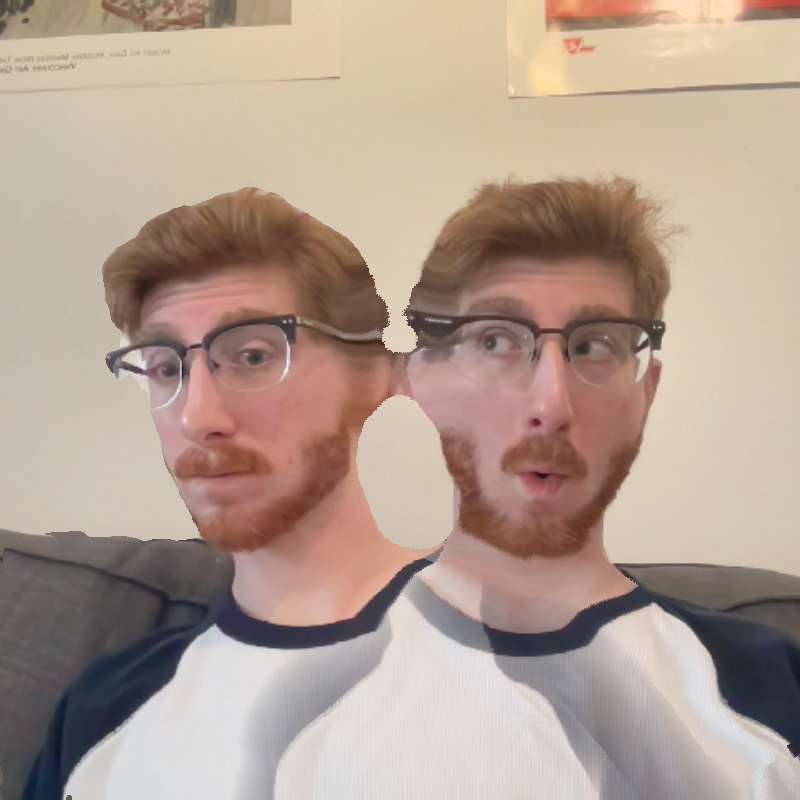
\includegraphics[width=0.45\linewidth]{img/merge2.png}
    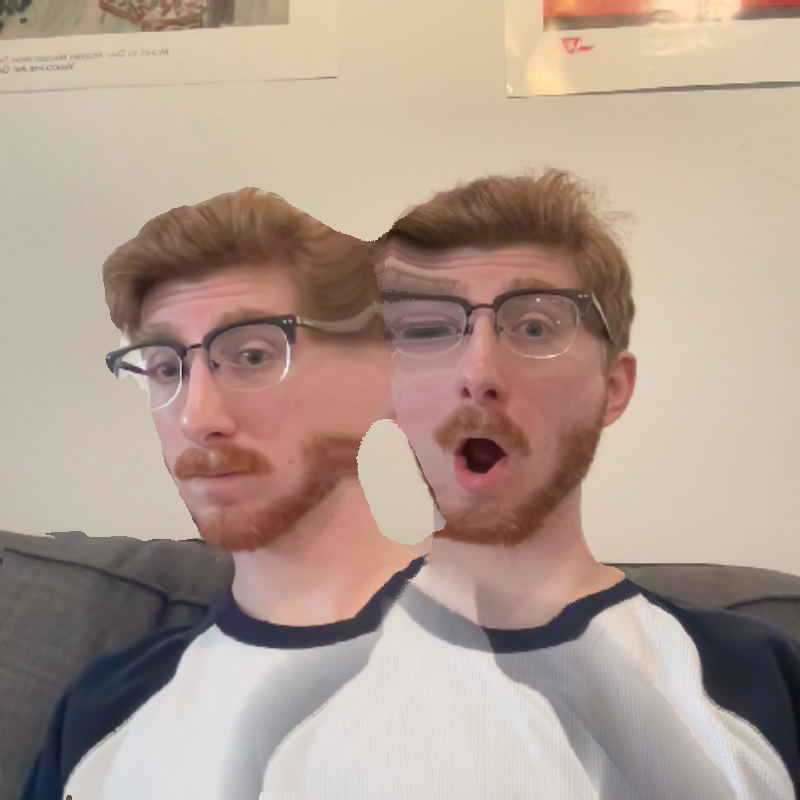
\includegraphics[width=0.45\linewidth]{img/merge3.png}
    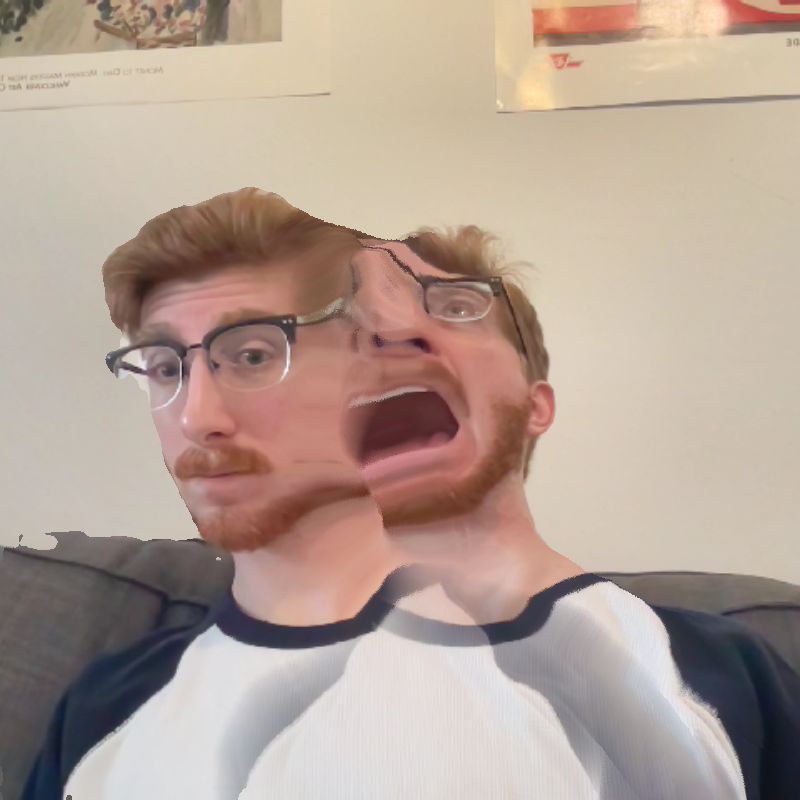
\includegraphics[width=0.45\linewidth]{img/merge4.png}
    \caption{As two subjects get closer together, distortion appears in the seam between them.}
    \label{fig:merge}
\end{figure}

\begin{figure}
    \centering
    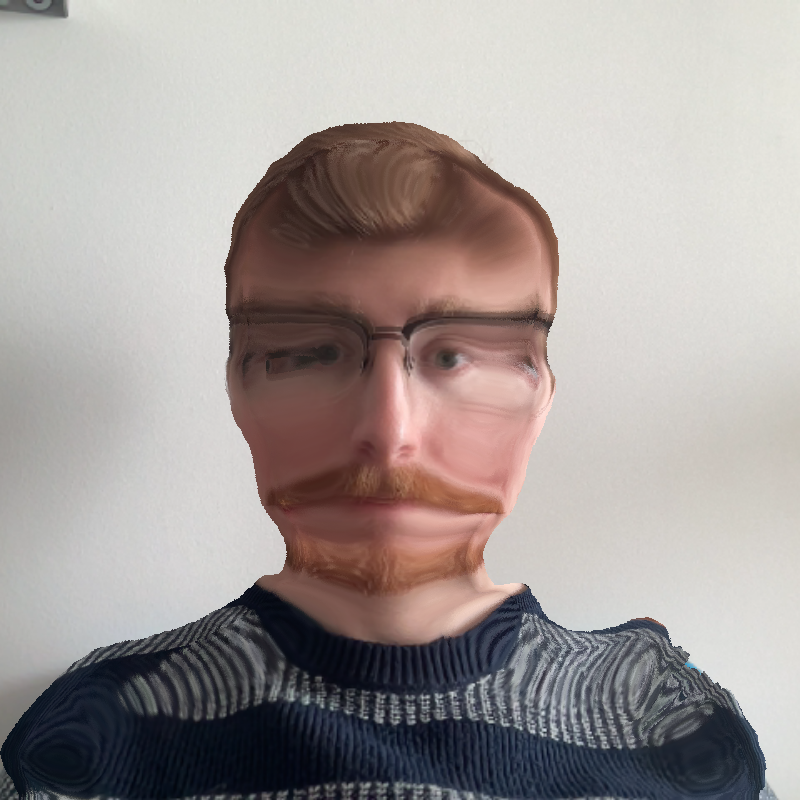
\includegraphics[width=0.65\linewidth]{img/overlap.png}
    \caption{When two subjects exactly overlap, their seams follows their contour. The whole contour is distorted, and their centers are undistorted.}
    \label{fig:overlap}
\end{figure}

We first create a signed distance $d_i$ ($i \in \{1,2\}$) to each subject by sampling pixel locations around the origin pixel $p_o$ to find the closest point $p_i$ on the edge of each subject. Since it is a signed distance, a negative distance implies that the current pixel is inside the subject, while a positive distance implies it is outside. We also create a signed distance to a smooth, merged shape, $d_m$, by using a smooth union operator~\cite{quilez-smin} that many scholars refer to as the ``bean operator.''~\cite{bean} We define a radius of influence $r$ to control the maximum distortion, leading to Equation~\ref{eq:dm} for the merged signed distance:

\begin{equation}
    \label{eq:dm}
    d_m = \min(d_1, d_2) - r\left(\frac{\max(4r-\vert d_1-d_2\vert, 0)}{4r}\right)^2
\end{equation}

The result of the smooth union distance is shown in Figure~\ref{fig:steps}g, with the boundary between red and blue showing the outline of the final shape.

If we were to grab color data from the input textures at the origin pixel coordinate, $\text{texture}(t_i, p_o)$, the original images would be reproduced undistorted. We want to start to smear them as they get close to each other, so we apply an offset to $p_o$ towards the closest edge. When a pixel on one subject is farther than $r$ away from the other subject, it should appear undistorted, so the magnitude is 0. When it is a distance of $r$ inside the other subject, it should also have a magnitude of 0. Where the subjects touch, there should be maximum distortion. The amount of distortion should smoothly interpolate between these extremes. We therefore base the magnitude based on the inverse of the absolute distance from any edge in Equation~\ref{eq:mag} and use it to offset the pixel coordinate used in a texture lookup in Equation~\ref{eq:ci}. The angle and magnitude of offset are shown in Figure~\ref{fig:steps}h,i.

\begin{align}
    \label{eq:mag}
    m &= r \prod_{i\in\{1,2\}}\left(1 - \left\vert \frac{d_i}{r} \right\vert\right) \\
    \label{eq:ci}
    c_i &= \text{texture}\left(t_i, p_o + m\frac{p_i-p_o}{\Vert p_i-p_o\Vert}\right)
\end{align}

We then produce the final output color by assigning a target weight to each input. Fully inside one subject, the target weight is 1, and right on the outside, the target weight is 0. To get the final merged color $c_m$, Equation~\ref{eq:cm} uses a linear combination of the source colors using normalized weights.

\begin{align}
    w_i &= \text{clamp}\left(\frac{d_i}{-r}, 0, 1\right) \\
    \label{eq:cm}
    c_m &= \frac{w_1}{w_1 + w_2}c_0 + \left(1 - \frac{w_1}{w_1 + w_2}\right)c_1
\end{align}

\section{Results and Analysis}

To evaluate Pandemonium, we asked users to take photos with it to see what creations they would make using the jank characteristics described in Section~\ref{sec:characteristics}.

Figure~\ref{fig:self} shows different approaches to the self portrait. Compared with a traditional headshot, these images shock the viewer and provide a significantly more memorable viewing experience. For this reason, Pandemonium self portraits make for great LinkedIn photos.

\begin{figure}
    \centering
    
\includegraphics[width=0.98\linewidth]{img/linkedin-zoom.png}
    \caption{Figure~\ref{fig:overlap} as a LinkedIn photo.}
    \label{fig:linkedin}
\end{figure}

Figure~\ref{fig:group} demonstrates the possibilities of group photos: when faces are unrecognizably smeared into each other, the result is much more memorable than a straightforward portrait would have been.

Figure~\ref{fig:temporal} shows use of duplication that creates a sense of progression using layering that would be impossible in a slit scan panorama. The left image creates a sense of anticipation before an action. The right image shows an Animorphs-style~\cite{hollister-2019} transformation from a regular human to a human eating noodles.

Finally, Figure~\ref{fig:feelings} exhibits the breadth of emotions possible by combining figures. The left image reminds the viewer of a yin/yang dichotomy, and the right image evokes papal or saintly feelings.

\begin{figure}
    \centering
    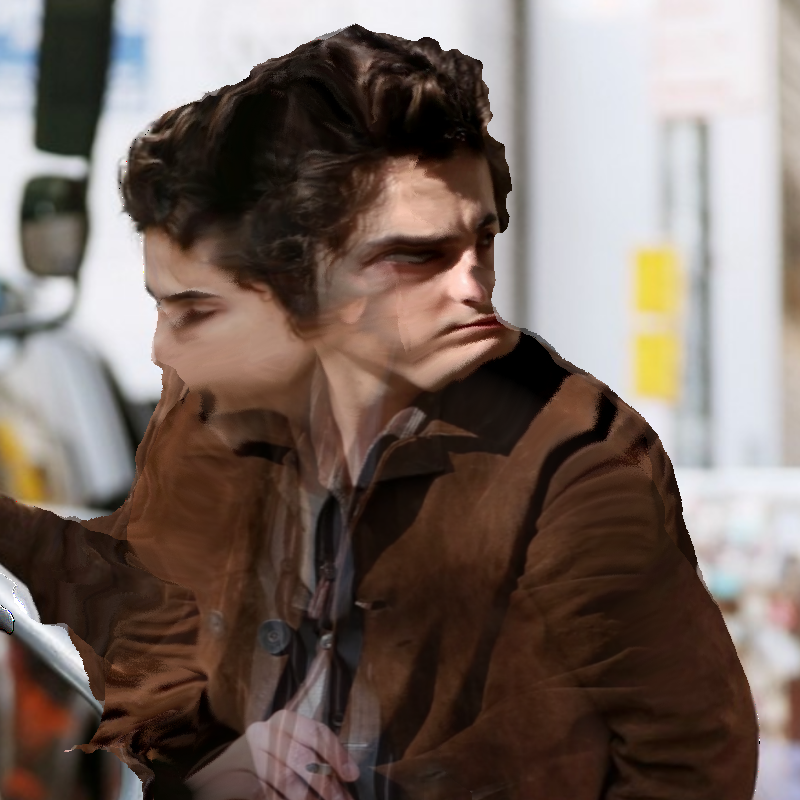
\includegraphics[width=0.48\linewidth]{img/timothee.png}
    \caption{A composite of two Timoth\'ee Chalamet pics from \textit{A Complete Unknown} (2024).}
    \label{fig:timothee}
\end{figure}

% \begin{figure}
%     \centering
%     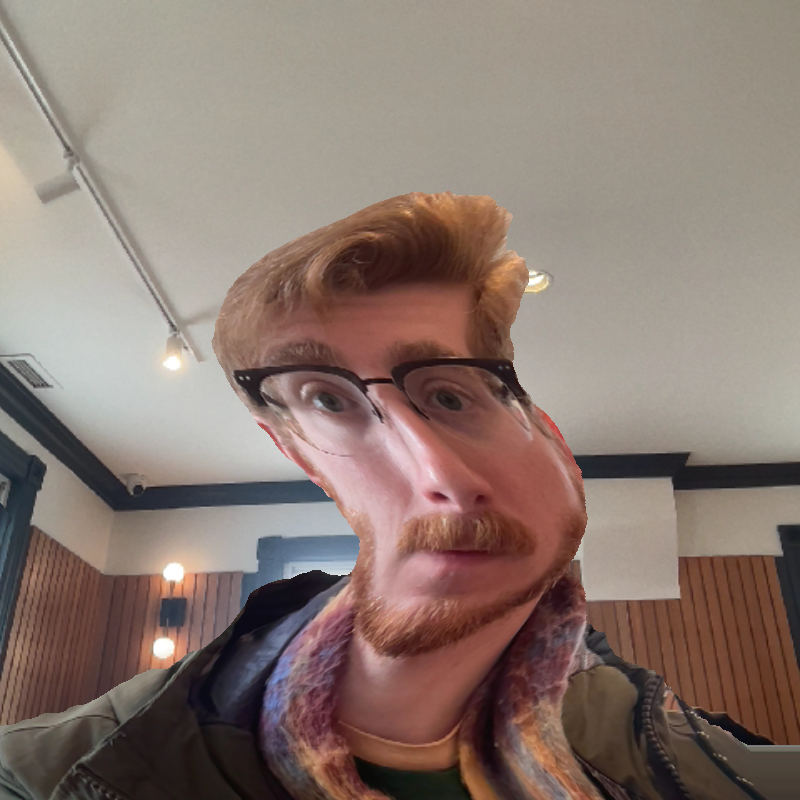
\includegraphics[width=0.5\linewidth]{img/warp.png}
%     \caption{Warped inputs}
%     \label{fig:warp}
% \end{figure}

\section{Conclusion}

Pandemonium breaks panorama apps out of a cycle of stagnation and creates truly memorable images. As Timoth\'ee Chalamet says in \textit{A Complete Unknown}~(2024), anyone who wants to attract attention has ``gotta be a freak.''~\cite{completeunknown} With Pandemonium, it's easier than ever to be a freak.

\begin{figure}
    \centering
    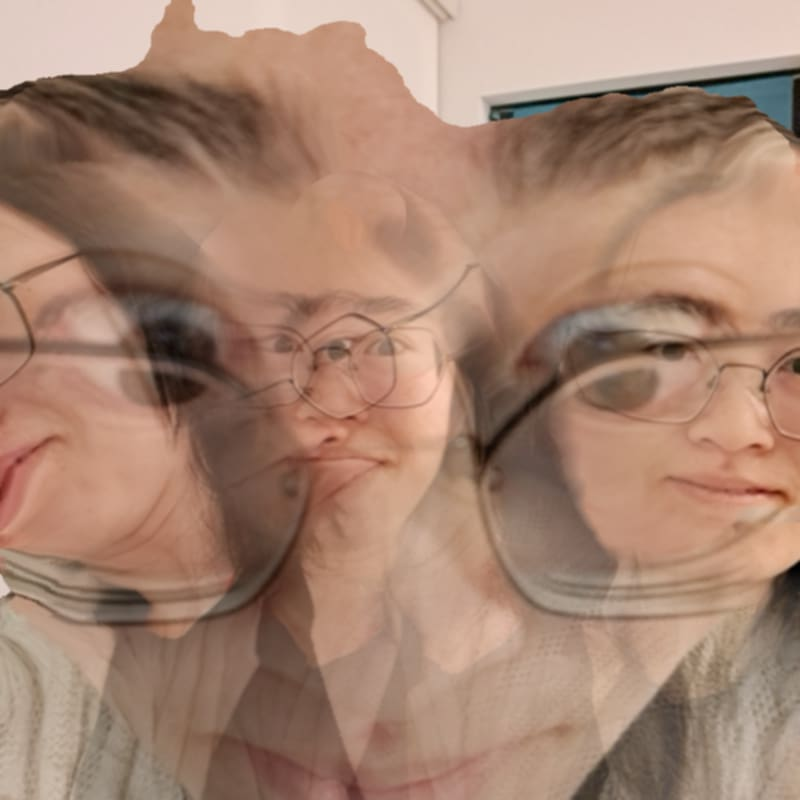
\includegraphics[width=0.48\linewidth]{img/anna.jpg}
    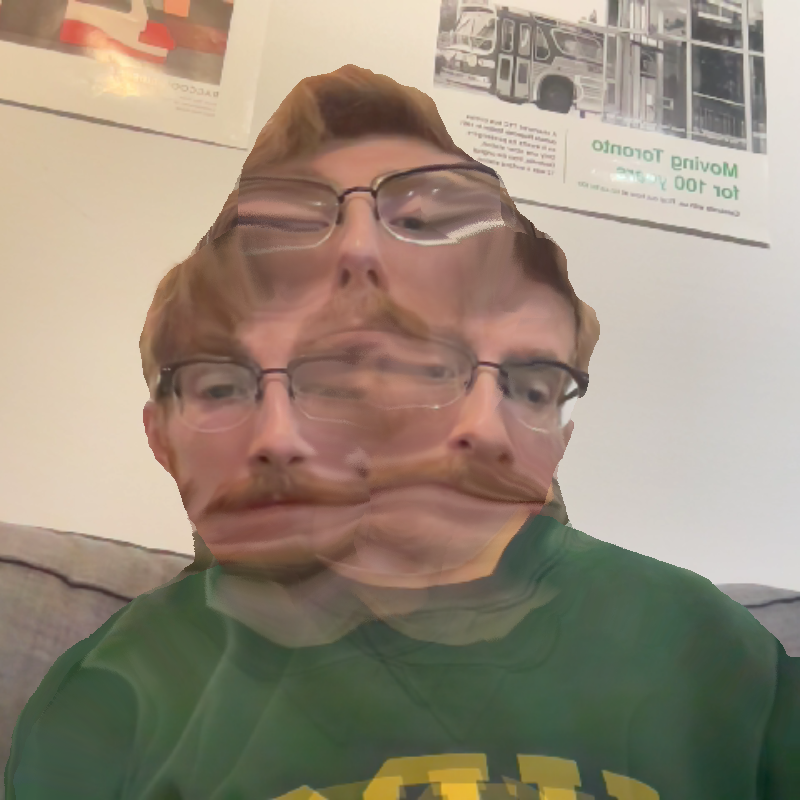
\includegraphics[width=0.48\linewidth]{img/cerberus.png}
    \caption{Self portraits using different forms of jank}
    \label{fig:self}
\end{figure}

\begin{figure}
    \centering
    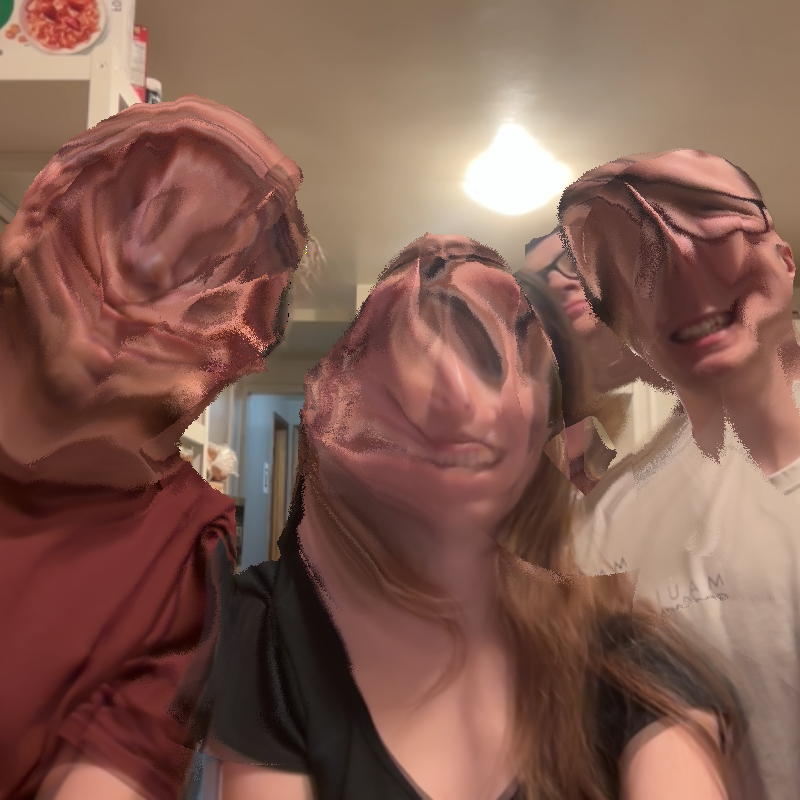
\includegraphics[width=0.48\linewidth]{img/faces.png}
    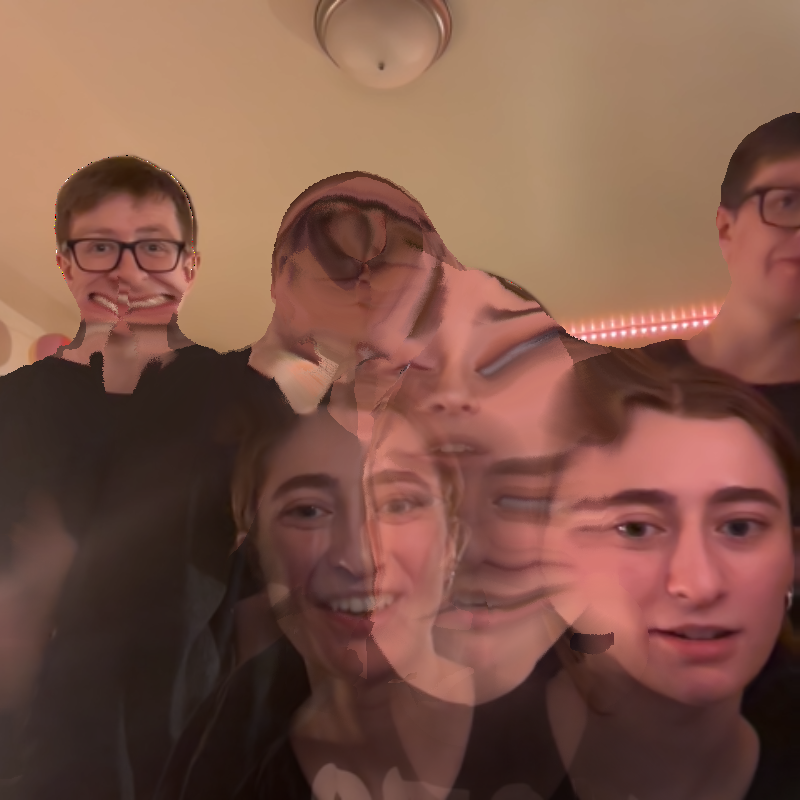
\includegraphics[width=0.48\linewidth]{img/pandemonium (1).png}
    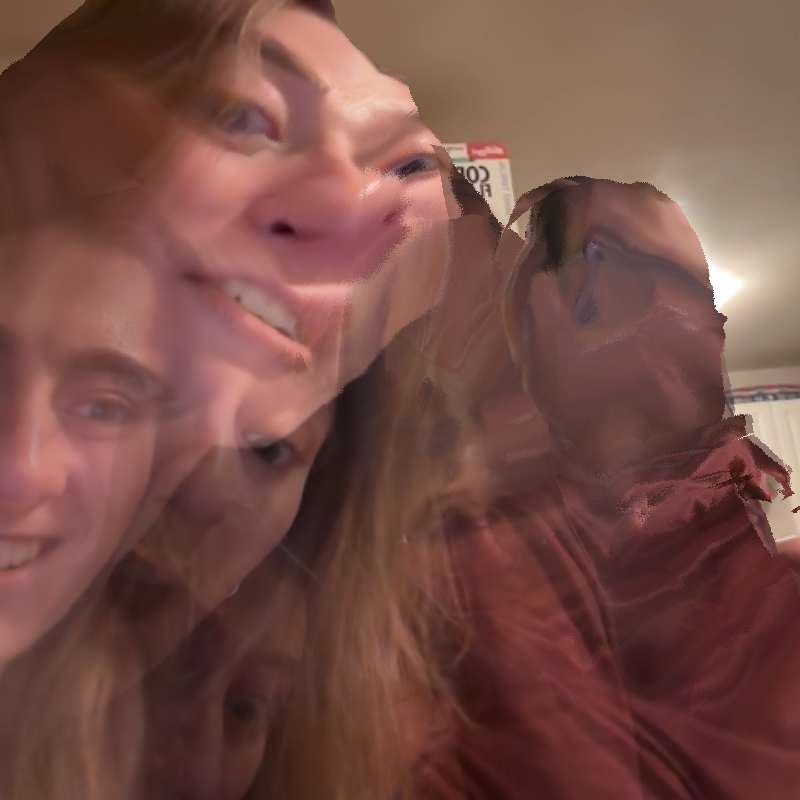
\includegraphics[width=0.48\linewidth]{img/bigsari.png}
    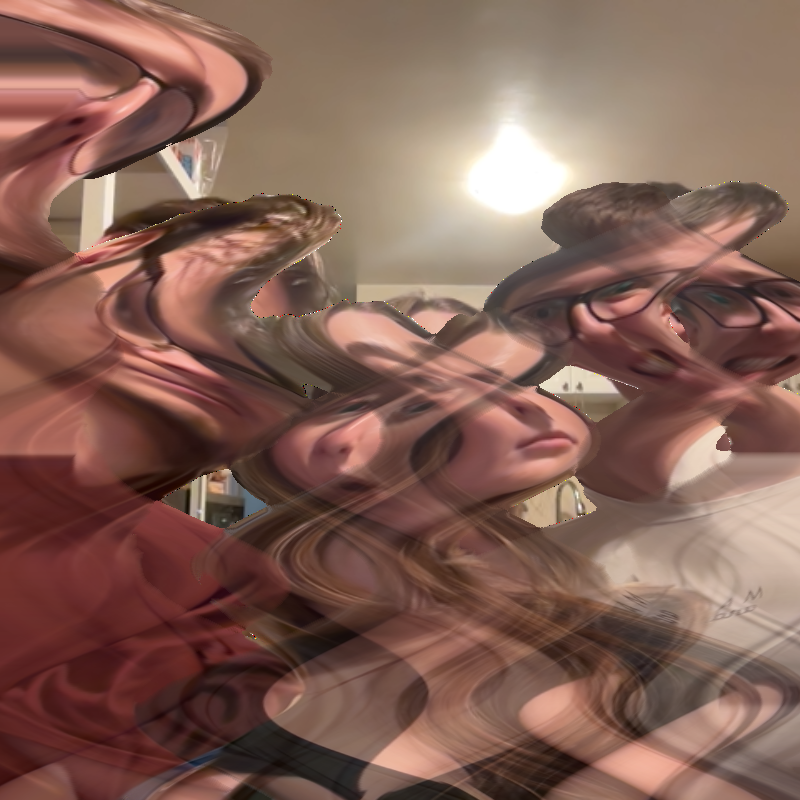
\includegraphics[width=0.48\linewidth]{img/wiggle.png}
    \caption{Group photos compositing multiple exposures of the same group}
    \label{fig:group}
\end{figure}

\begin{figure}
    \centering
    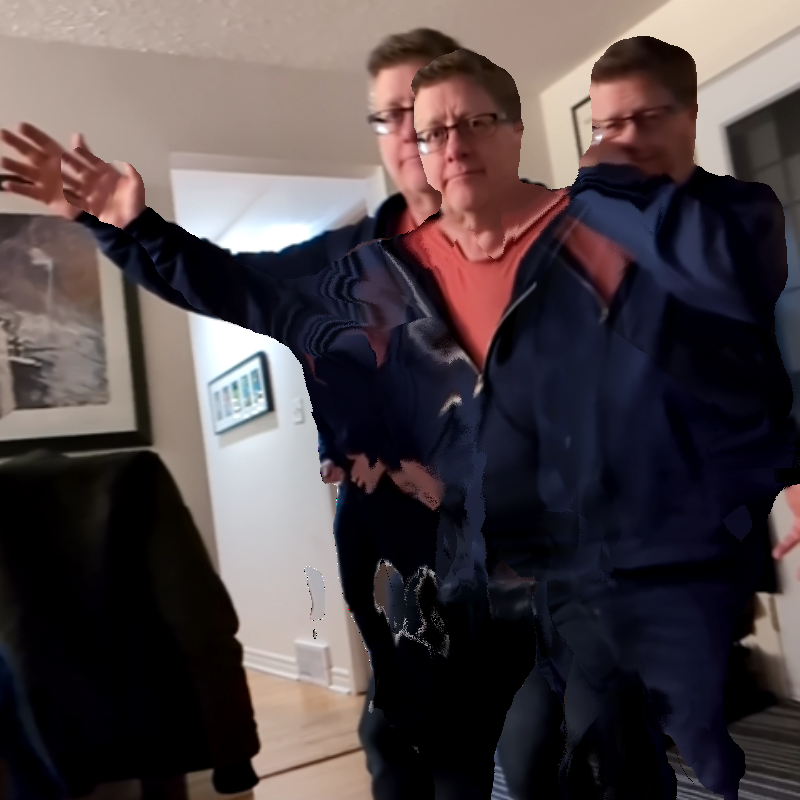
\includegraphics[width=0.48\linewidth]{img/dad.png}
    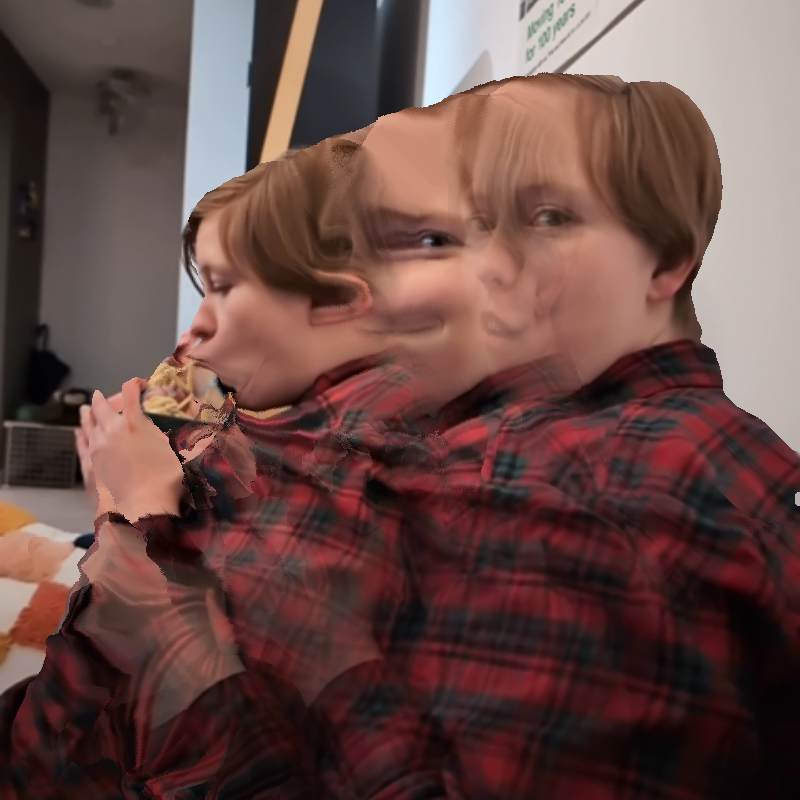
\includegraphics[width=0.48\linewidth]{img/noodles.png}
    \caption{Uses of duplication to create unique effects}
    \label{fig:temporal}
\end{figure}

\begin{figure}
    \centering
    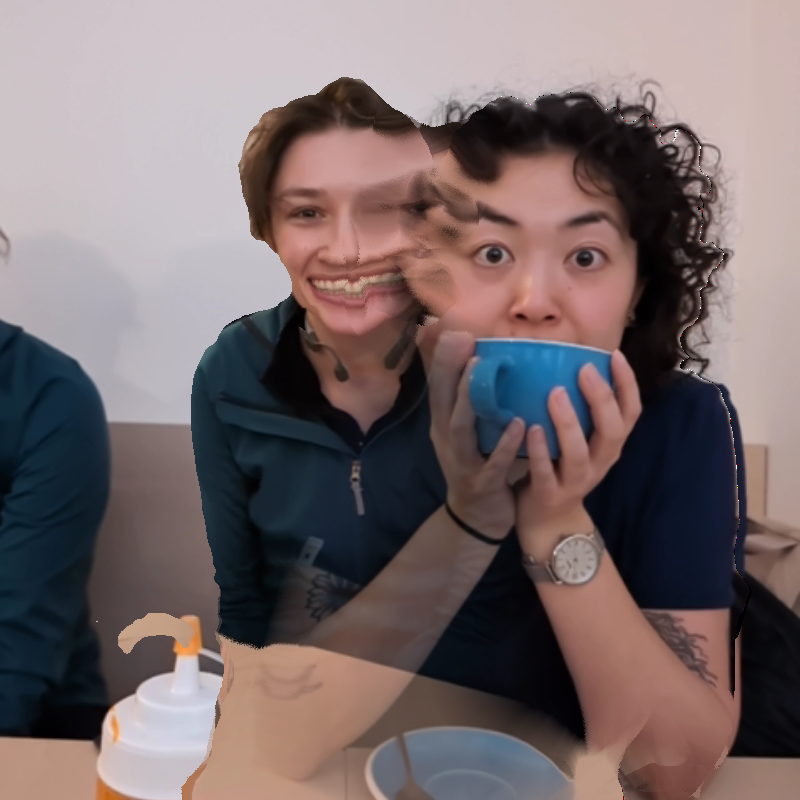
\includegraphics[width=0.48\linewidth]{img/sitzi.png}
    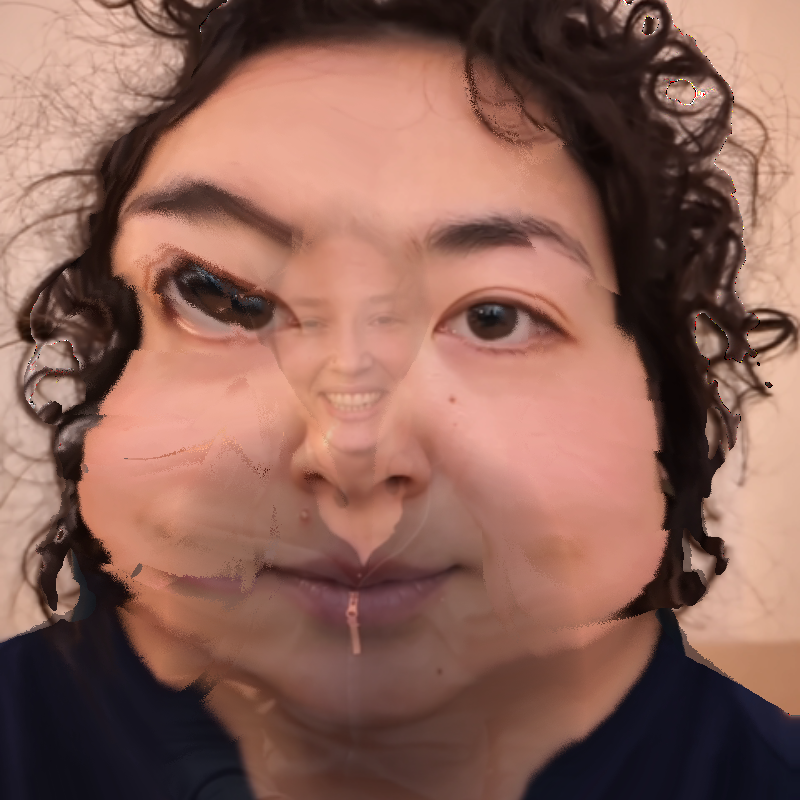
\includegraphics[width=0.48\linewidth]{img/marah.png}
    \caption{How do these images make you feel?}
    \label{fig:feelings}
\end{figure}

\bibliographystyle{plainurl}
\bibliography{main}

\end{document}
